\chapter{RESULTADOS E DISCUSSÃO}
\label{cap:resultados}

Este capítulo reúne os resultados das três campanhas experimentais. A primeira estabelece a comparação entre CUBIC, BBR e CUBIC-RTT em condições controladas. A segunda verifica como a proposta se comporta quando a capacidade do gargalo, o número de fluxos e os coeficientes de adaptação são modificados. A terceira coloca CUBIC e CUBIC-RTT em competição direta, permitindo observar se a adaptação altera a divisão da capacidade disponível entre fluxos de algoritmos diferentes.

As médias apresentadas são descritivas. Como algumas configurações produziram resultados idênticos entre repetições, não se atribui significância estatística às diferenças sem uma fonte efetiva de variabilidade. As barras de erro dos gráficos representam a dispersão observada entre as execuções consideradas.

\section{Comparação Inicial entre CUBIC, BBR e CUBIC-RTT}

A campanha inicial utilizou quatro fluxos TCP concorrentes, gargalo de 2 Mbps, enlaces de acesso de 10 Mbps com atraso de 45 ms e duração de 100 segundos por execução. Foram avaliados atrasos de gargalo de 10 ms, 50 ms e 100 ms, com cinco repetições por algoritmo e cenário, totalizando 45 simulações.

A Tabela~\ref{tab:resultados-iniciais} apresenta as médias das cinco execuções. A vazão corresponde à taxa agregada de dados úteis recebidos, e o atraso é o unidirecional, obtido pelo FlowMonitor.

\begin{table}[htbp]
\centering
\caption{Médias da campanha comparativa inicial}
\label{tab:resultados-iniciais}
\small
\begin{tabular}{c l r r r r}
\toprule
\textbf{Atraso} & \textbf{Algoritmo} & \textbf{Vazão (Mbps)} & \textbf{Perda (\%)} & \textbf{Atraso (ms)} & \textbf{Jitter (ms)} \\
\midrule
10 ms & CUBIC & 1,980 & 1,43 & 311,71 & 1,632 \\
10 ms & CUBIC-RTT & 1,980 & 1,42 & 319,91 & 1,610 \\
10 ms & BBR & 1,942 & 17,58 & 337,51 & 1,060 \\
\midrule
50 ms & CUBIC & 1,968 & 1,90 & 409,79 & 1,650 \\
50 ms & CUBIC-RTT & 1,966 & 2,00 & 419,28 & 1,595 \\
50 ms & BBR & 1,926 & 18,35 & 449,15 & 1,100 \\
\midrule
100 ms & CUBIC & 1,968 & 2,26 & 532,50 & 1,718 \\
100 ms & CUBIC-RTT & 1,968 & 2,46 & 545,39 & 1,659 \\
100 ms & BBR & 1,917 & 19,32 & 583,06 & 1,190 \\
\bottomrule
\end{tabular}
\end{table}

\subsection{Vazão e perda de pacotes}

CUBIC e CUBIC-RTT atingiram vazões agregadas praticamente iguais nos três atrasos. A diferença máxima foi de 0,002 Mbps no cenário de 50 ms. Isso indica que, nessa configuração, a introdução da adaptação baseada em RTT não comprometeu a utilização agregada do gargalo.

A perda de pacotes, por outro lado, não apresentou uma vantagem uniforme. Em 10 ms, CUBIC-RTT registrou 1,42\%, ligeiramente abaixo dos 1,43\% do CUBIC. Em 50 ms, a perda foi de 2,00\% para a proposta e 1,90\% para o algoritmo original. Em 100 ms, os valores foram 2,46\% e 2,26\%, respectivamente. A diferença é pequena em termos absolutos, mas mostra que a adaptação não reduziu as perdas em todas as condições.

O BBR apresentou perda consideravelmente maior nos três cenários, entre 17,58\% e 19,32\%. Esse comportamento deve ser interpretado no contexto da topologia, dos buffers e da configuração utilizada. Ele não permite concluir que o BBR apresente necessariamente esse nível de perda em outras versões ou ambientes.

\begin{figure}[htbp]
\centering
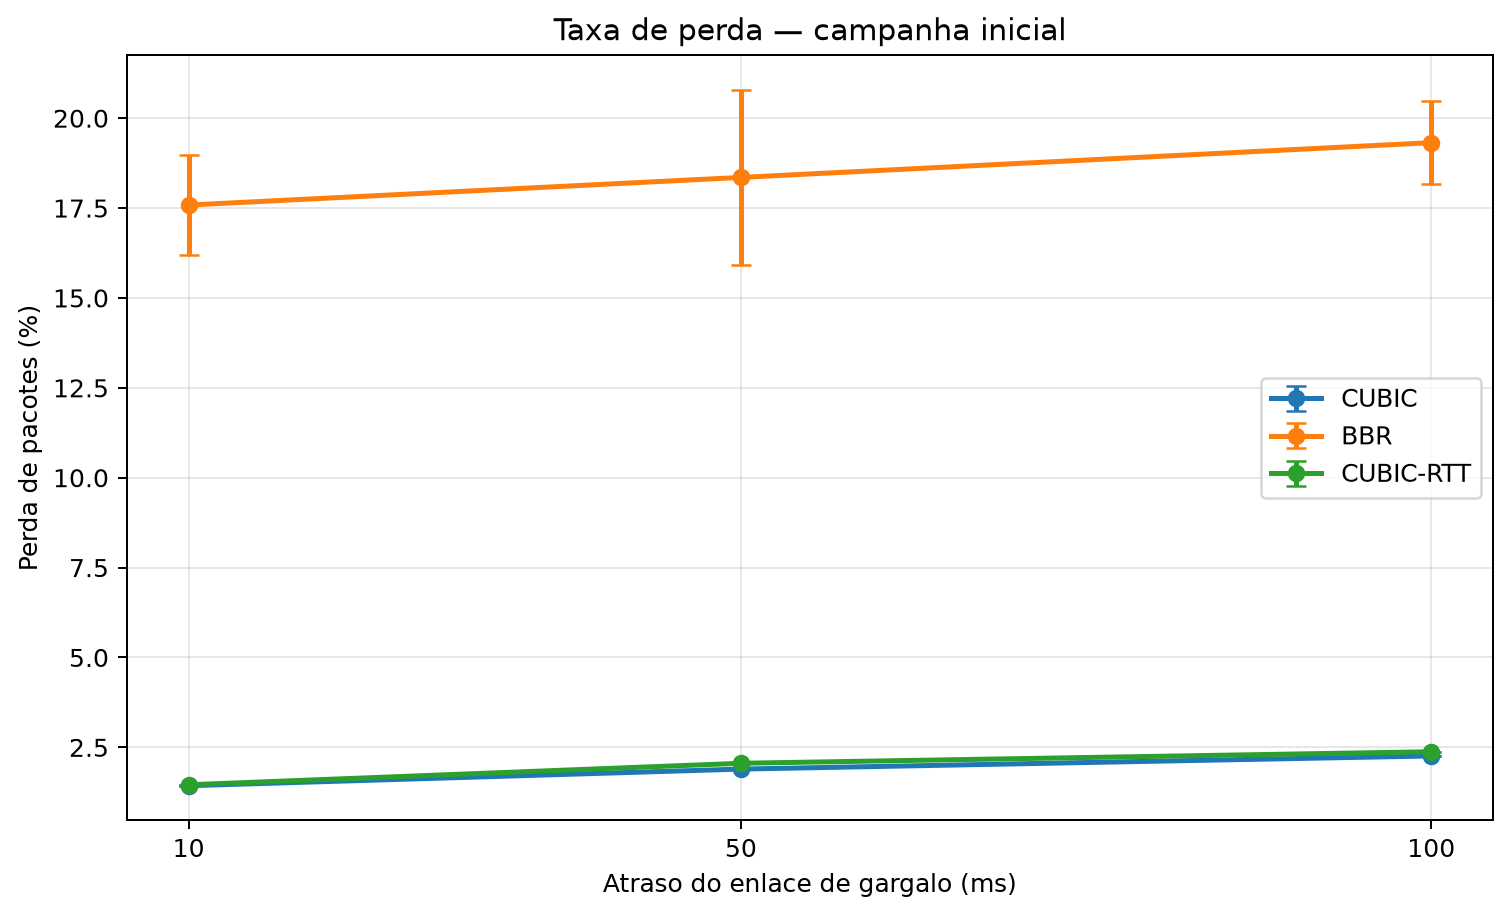
\includegraphics[width=0.88\textwidth]{inicial_packet_loss.png}
\caption{Taxa de perda de pacotes na campanha inicial.}
\label{fig:inicial-perda}
\end{figure}

\subsection{Atraso médio e RTT}

O atraso médio unidirecional aumentou à medida que o atraso configurado no gargalo passou de 10 ms para 100 ms. Para o CUBIC, as médias foram 311,71 ms, 409,79 ms e 532,50 ms. Para o CUBIC-RTT, foram 319,91 ms, 419,28 ms e 545,39 ms. Em todos os cenários, portanto, a proposta apresentou atraso médio superior, com diferenças de 8,20 ms, 9,49 ms e 12,89 ms.

Esse resultado é importante porque delimita o alcance da hipótese inicial. A utilização de RTT na adaptação não produziu, nessa campanha, uma redução do atraso médio de entrega. O mecanismo considera o menor RTT observado em relação a uma referência, e não atua diretamente sobre cada aumento instantâneo de atraso provocado pelo enfileiramento.

\begin{figure}[htbp]
\centering
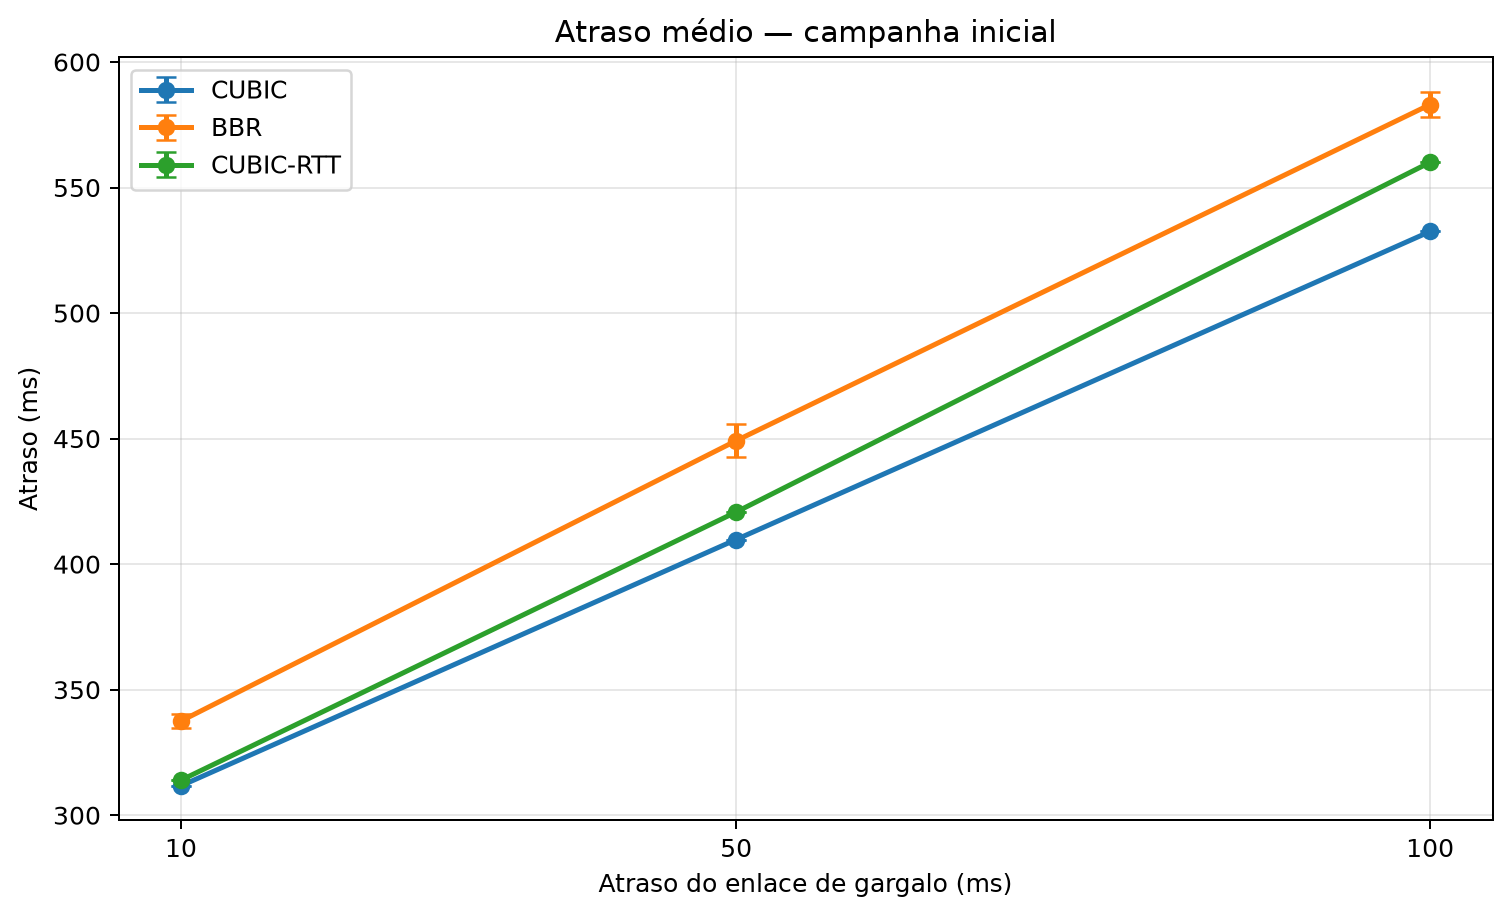
\includegraphics[width=0.88\textwidth]{inicial_delay.png}
\caption{Atraso médio unidirecional na campanha inicial.}
\label{fig:inicial-atraso}
\end{figure}

O gráfico de RTT médio complementa essa leitura, pois apresenta a medida de ida e volta observada pela conexão, distinta do atraso unidirecional do FlowMonitor. As duas métricas não são intercambiáveis: a primeira alimenta a lógica adaptativa do CUBIC-RTT, enquanto a segunda descreve o tempo de entrega dos pacotes em um sentido.

\begin{figure}[htbp]
\centering
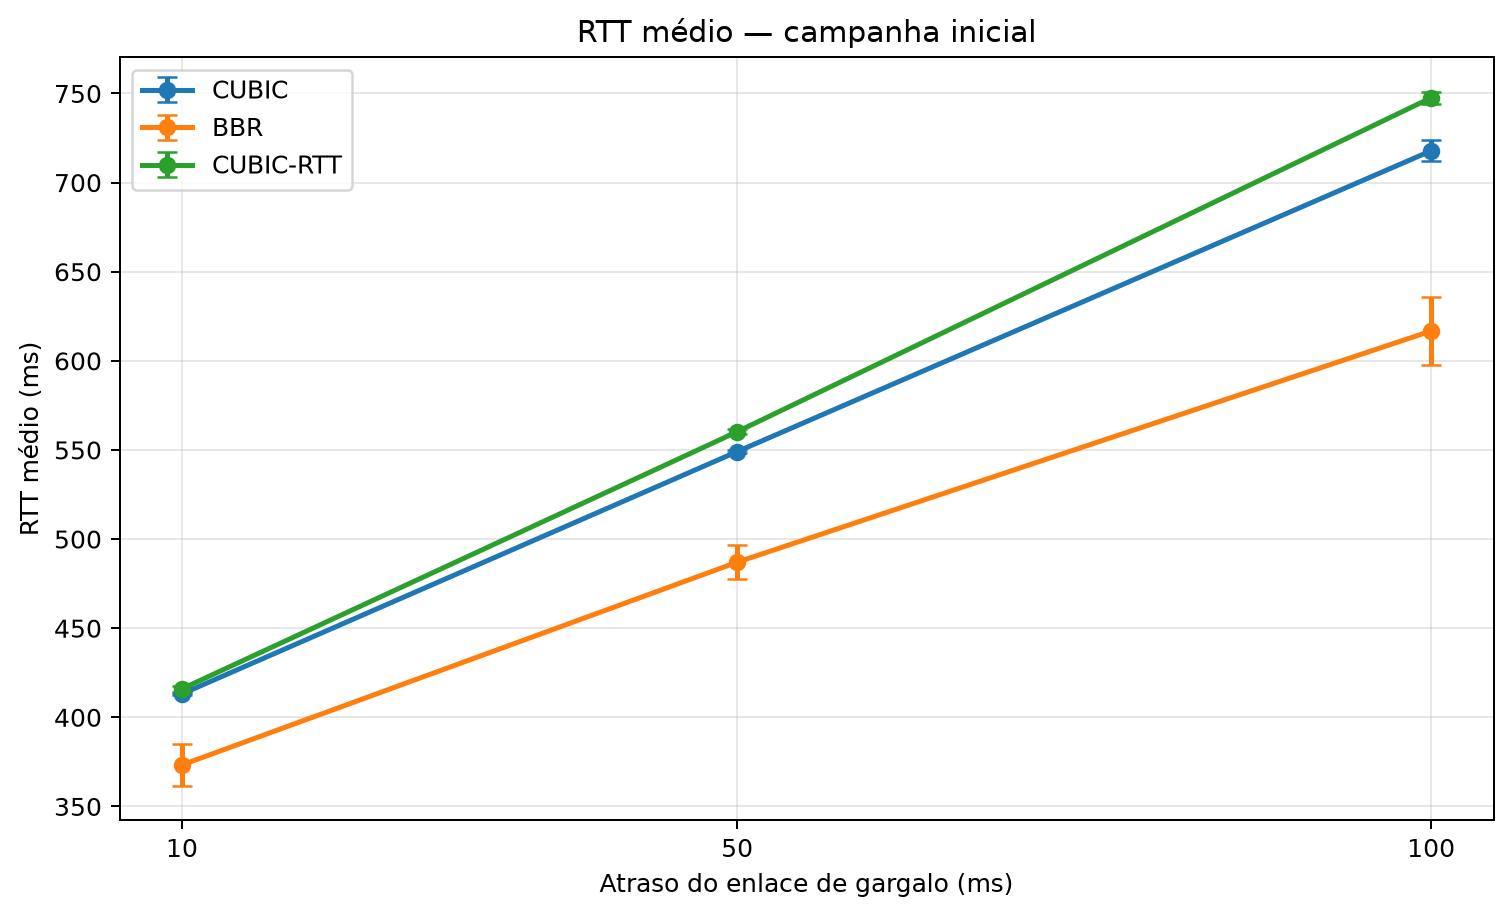
\includegraphics[width=0.88\textwidth]{inicial_rtt.png}
\caption{RTT médio observado na campanha inicial.}
\label{fig:inicial-rtt}
\end{figure}

\subsection{Jitter}

O resultado mais favorável ao CUBIC-RTT na comparação inicial foi o jitter. A proposta registrou 1,610 ms, 1,595 ms e 1,659 ms, enquanto o CUBIC apresentou 1,632 ms, 1,650 ms e 1,718 ms. As reduções foram de aproximadamente 1,3\%, 3,3\% e 3,4\%.

As diferenças absolutas são moderadas, mas mantêm o mesmo sentido nos três atrasos avaliados. O BBR apresentou jitter ainda menor, entre 1,060 ms e 1,190 ms, mas esse resultado ocorreu junto de perdas de pacotes muito superiores às observadas nos dois algoritmos CUBIC.

\begin{figure}[htbp]
\centering
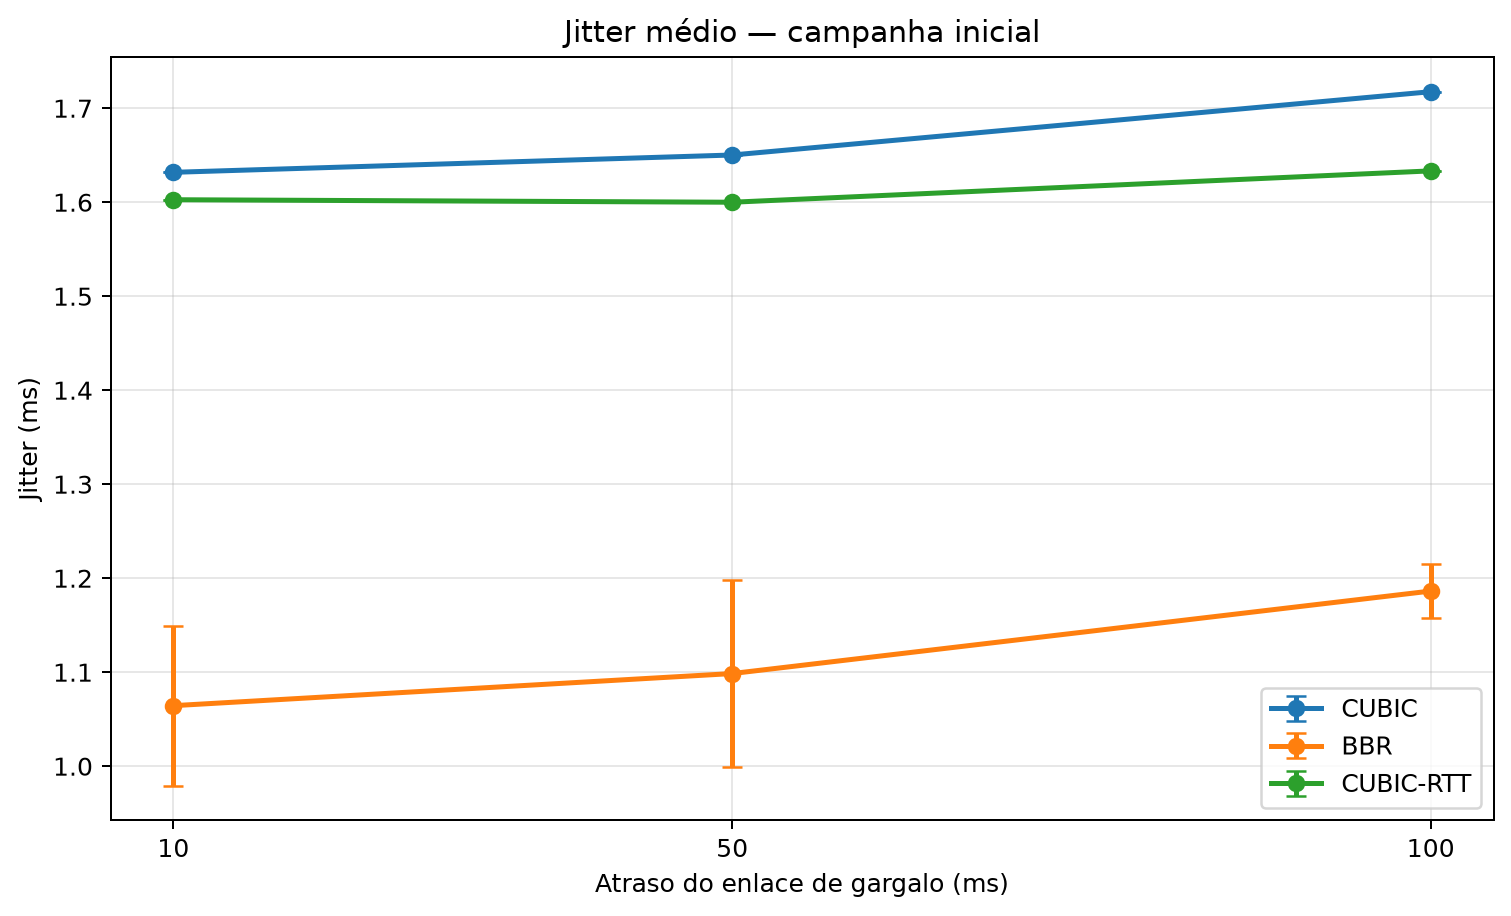
\includegraphics[width=0.88\textwidth]{inicial_jitter.png}
\caption{Jitter médio na campanha inicial.}
\label{fig:inicial-jitter}
\end{figure}

Em resumo, os resultados iniciais indicam que a adaptação pode alterar a regularidade temporal da entrega sem reduzir a vazão agregada. Essa mudança, porém, não veio acompanhada de menor atraso ou menor perda de forma consistente. A primeira campanha sustenta a hipótese de que informações de RTT influenciam o comportamento do CUBIC, mas não demonstra melhoria global em todas as métricas.

\section{Campanha de Robustez e Variação de Parâmetros}

A campanha de robustez reuniu 675 simulações, distribuídas em três cenários de rede, quinze configurações de algoritmo e parâmetros, três atrasos de gargalo e cinco repetições. Foram avaliados o CUBIC original, o BBR e treze configurações do CUBIC-RTT, incluindo a configuração de referência ($\alpha=0{,}25$ e $\gamma=0{,}05$).

Os mapas de calor preservados no projeto permitem examinar em detalhe os cenários \texttt{bw1\_f4} e \texttt{bw2\_f8}. O cenário \texttt{access100} também integrou a matriz de execução e a auditoria estrutural, mas não possui, no conjunto de figuras desta versão, mapas equivalentes que permitam uma discussão numérica com o mesmo nível de detalhe. Por isso, a comparação quantitativa a seguir concentra-se nos dois cenários com resultados gráficos disponíveis.

\subsection{Cenário bw1\_f4: gargalo de 1 Mbps e quatro fluxos}

Nesse cenário, a vazão permaneceu próxima de 0,99 Mbps para o CUBIC e para todas as configurações CUBIC-RTT, independentemente do atraso do gargalo. Isso indica que a capacidade disponível foi praticamente toda utilizada e que a variação de $\alpha$ e $\gamma$ não produziu diferenças relevantes na vazão agregada.

As diferenças aparecem com maior clareza nas demais métricas. Com 100 ms de atraso, o CUBIC apresentou perda de 3,52\%, atraso médio de 652,12 ms, jitter de 3,57 ms e índice de Jain de 0,97. A configuração de referência do CUBIC-RTT apresentou, no mesmo cenário, perda de 4,11\%, atraso de 661,68 ms, jitter de 3,53 ms e índice de Jain de 0,99. Houve, então, pequena redução de jitter e melhor distribuição entre os fluxos, mas com aumento da perda e do atraso médio.

A variação dos coeficientes mostra que não existe uma combinação que minimize simultaneamente todas as métricas. Por exemplo, com 100 ms, a configuração $\alpha=0{,}50$ e $\gamma=0{,}025$ apresentou atraso médio de 633,86 ms, abaixo dos 652,12 ms do CUBIC. Entretanto, sua perda foi de 4,75\%, superior aos 3,52\% do algoritmo original, e o jitter chegou a 3,69 ms. Já a configuração $\alpha=0{,}10$ e $\gamma=0$ obteve atraso de 641,33 ms e perda de 3,83\%, combinando menor atraso que o CUBIC com perda um pouco maior.

O BBR manteve vazão próxima de 0,97 Mbps, mas apresentou perdas de 4,30\%, 17,70\% e 18,57\% nos três atrasos. Seu índice de Jain caiu para 0,65 em 50 ms e 0,82 em 100 ms. Novamente, esses números caracterizam o cenário simulado, não uma propriedade universal do BBR.

\subsection{Cenário bw2\_f8: gargalo de 2 Mbps e oito fluxos}

Com oito fluxos concorrentes e gargalo de 2 Mbps, a vazão também permaneceu próxima da capacidade disponível. CUBIC e CUBIC-RTT registraram aproximadamente 1,98 Mbps em 10 ms e 1,97 Mbps em 50 ms e 100 ms. A mudança dos coeficientes teve pouco efeito sobre essa métrica agregada.

A diferença entre as configurações voltou a aparecer no atraso, no jitter, na perda e na justiça. Com 100 ms, o CUBIC apresentou atraso médio de 548,06 ms, jitter de 2,19 ms, perda de 2,76\% e índice de Jain de 0,96. A configuração de referência do CUBIC-RTT apresentou atraso de 556,43 ms, jitter de 2,18 ms, perda de 3,21\% e índice de Jain de 0,94. Nesse caso, a pequena redução de jitter veio acompanhada de aumento do atraso e da perda e de uma distribuição um pouco menos equilibrada.

Algumas combinações produziram compromissos diferentes. A configuração $\alpha=0{,}10$ e $\gamma=0{,}10$, por exemplo, reduziu o jitter para 1,90 ms, 1,87 ms e 1,93 ms nos três atrasos, abaixo dos valores do CUBIC. Em contrapartida, com 100 ms, seu atraso médio foi de 578,82 ms e a perda foi de 3,11\%, ambos superiores aos do algoritmo original. Por outro lado, configurações com $\gamma=0$ chegaram a apresentar atraso médio menor em 100 ms, mas sem manter a mesma vantagem em jitter e perda.

O BBR apresentou perdas entre 20,15\% e 21,48\% e índices de Jain entre 0,46 e 0,74. Embora sua vazão tenha permanecido próxima de 1,93--1,95 Mbps, a distribuição entre os oito fluxos foi consideravelmente menos equilibrada nesse cenário específico.

\subsection{Influência dos coeficientes \texorpdfstring{$\alpha$ e $\gamma$}{alpha e gamma}}

Os mapas de calor mostram que a influência dos coeficientes depende do cenário e da métrica observada. O coeficiente $\alpha$ altera a intensidade da adaptação do fator cúbico $C$, afetando o crescimento da janela. O coeficiente $\gamma$ modula a alteração de $\beta$ após a perda. Como os dois mecanismos atuam em momentos diferentes do controle de congestionamento, seus efeitos não precisam aparecer simultaneamente nem na mesma direção em todas as métricas.

De forma geral, a vazão agregada permaneceu próxima ao limite do gargalo em quase todas as configurações. Isso significa que a comparação entre parâmetros é mais informativa quando se observam atraso, jitter, perda e justiça. Em algumas condições, determinadas combinações reduziram o atraso ou o jitter, mas aumentaram a perda de pacotes; em outras, melhoraram o índice de Jain sem oferecer vantagem de vazão. A configuração de referência, portanto, deve ser entendida como um ponto de partida para a avaliação, e não como uma escolha ótima para todos os cenários.

A campanha de robustez reforça a conclusão da comparação inicial: a adaptação baseada em RTT modifica o comportamento do CUBIC e pode favorecer uma métrica em determinadas condições, mas o efeito não é uniforme. Não foi identificada uma combinação de $\alpha$ e $\gamma$ que dominasse o CUBIC original em vazão, atraso, jitter, perda e justiça ao mesmo tempo.

\section{Coexistência entre Fluxos CUBIC e CUBIC-RTT}

A campanha de coexistência avalia uma questão diferente das comparações anteriores: não apenas como cada algoritmo se comporta isoladamente, mas como os dois disputam a mesma capacidade de transmissão. Foram utilizados oito fluxos simultâneos, quatro CUBIC e quatro CUBIC-RTT, com a mesma configuração de referência da proposta ($\alpha=0{,}25$ e $\gamma=0{,}05$). Os enlaces de acesso foram distribuídos em pares com atrasos de 10 ms, 30 ms, 60 ms e 90 ms, enquanto o gargalo de 10 Mbps foi avaliado com atrasos de 10 ms, 50 ms e 100 ms.

A Tabela~\ref{tab:coexistencia} apresenta a vazão média por fluxo, o atraso médio, o jitter e a perda de cada grupo. Para cada repetição, foram calculadas as médias dos quatro fluxos pertencentes ao mesmo algoritmo; em seguida, foram calculadas as médias das cinco repetições. A perda foi consolidada pela razão entre pacotes perdidos e pacotes transmitidos.

\begin{table}[htbp]
\centering
\caption{Resultados médios da campanha de coexistência}
\label{tab:coexistencia}
\small
\resizebox{\textwidth}{!}{
\begin{tabular}{c l r r r r}
\toprule
\textbf{Atraso do gargalo} & \textbf{Algoritmo} & \textbf{Vazão por fluxo (Mbps)} & \textbf{Perda (\%)} & \textbf{Atraso médio (ms)} & \textbf{Jitter (ms)} \\
\midrule
10 ms & CUBIC & 1,2492 & 0,2465 & 450,008 & 0,6100 \\
10 ms & CUBIC-RTT & 1,2345 & 0,2416 & 449,700 & 0,6131 \\
\midrule
50 ms & CUBIC & 1,2068 & 0,3229 & 552,776 & 0,6487 \\
50 ms & CUBIC-RTT & 1,2757 & 0,3177 & 552,603 & 0,6380 \\
\midrule
100 ms & CUBIC & 1,1070 & 0,5070 & 678,778 & 0,7060 \\
100 ms & CUBIC-RTT & 1,3746 & 0,4590 & 678,291 & 0,6556 \\
\bottomrule
\end{tabular}}
\end{table}

\subsection{Vazão: redistribuição da capacidade entre os algoritmos}

Com atraso de gargalo de 10 ms, a vazão média por fluxo CUBIC foi de 1,2492 Mbps, ligeiramente superior aos 1,2345 Mbps do CUBIC-RTT. A diferença representa aproximadamente 1,2\%. Em 50 ms, a relação se inverteu: o CUBIC-RTT alcançou 1,2757 Mbps por fluxo, contra 1,2068 Mbps do CUBIC, uma vantagem de aproximadamente 5,7\%.

A diferença ficou mais evidente em 100 ms. O CUBIC-RTT atingiu 1,3746 Mbps por fluxo, enquanto o CUBIC caiu para 1,1070 Mbps, o que representa uma vantagem de aproximadamente 24,2\% para a variante adaptativa. Como cada algoritmo possui quatro fluxos, a vazão total da rede permaneceu próxima de 9,93 Mbps nos três cenários. Na prática, o aumento da vazão do CUBIC-RTT não representa um crescimento equivalente da capacidade total utilizada: representa principalmente uma redistribuição da banda em favor dos fluxos que executam a proposta.

A participação do CUBIC-RTT na vazão total passou de aproximadamente 49,7\% em 10 ms para 51,4\% em 50 ms e 55,4\% em 100 ms. Esse resultado é central para a avaliação da hipótese: a adaptação pode manter a utilização do gargalo e, ao mesmo tempo, tornar o CUBIC-RTT mais competitivo que o CUBIC original quando os atrasos aumentam. Isso também significa que a proposta não é neutra em relação a fluxos CUBIC concorrentes.

\begin{figure}[htbp]
\centering
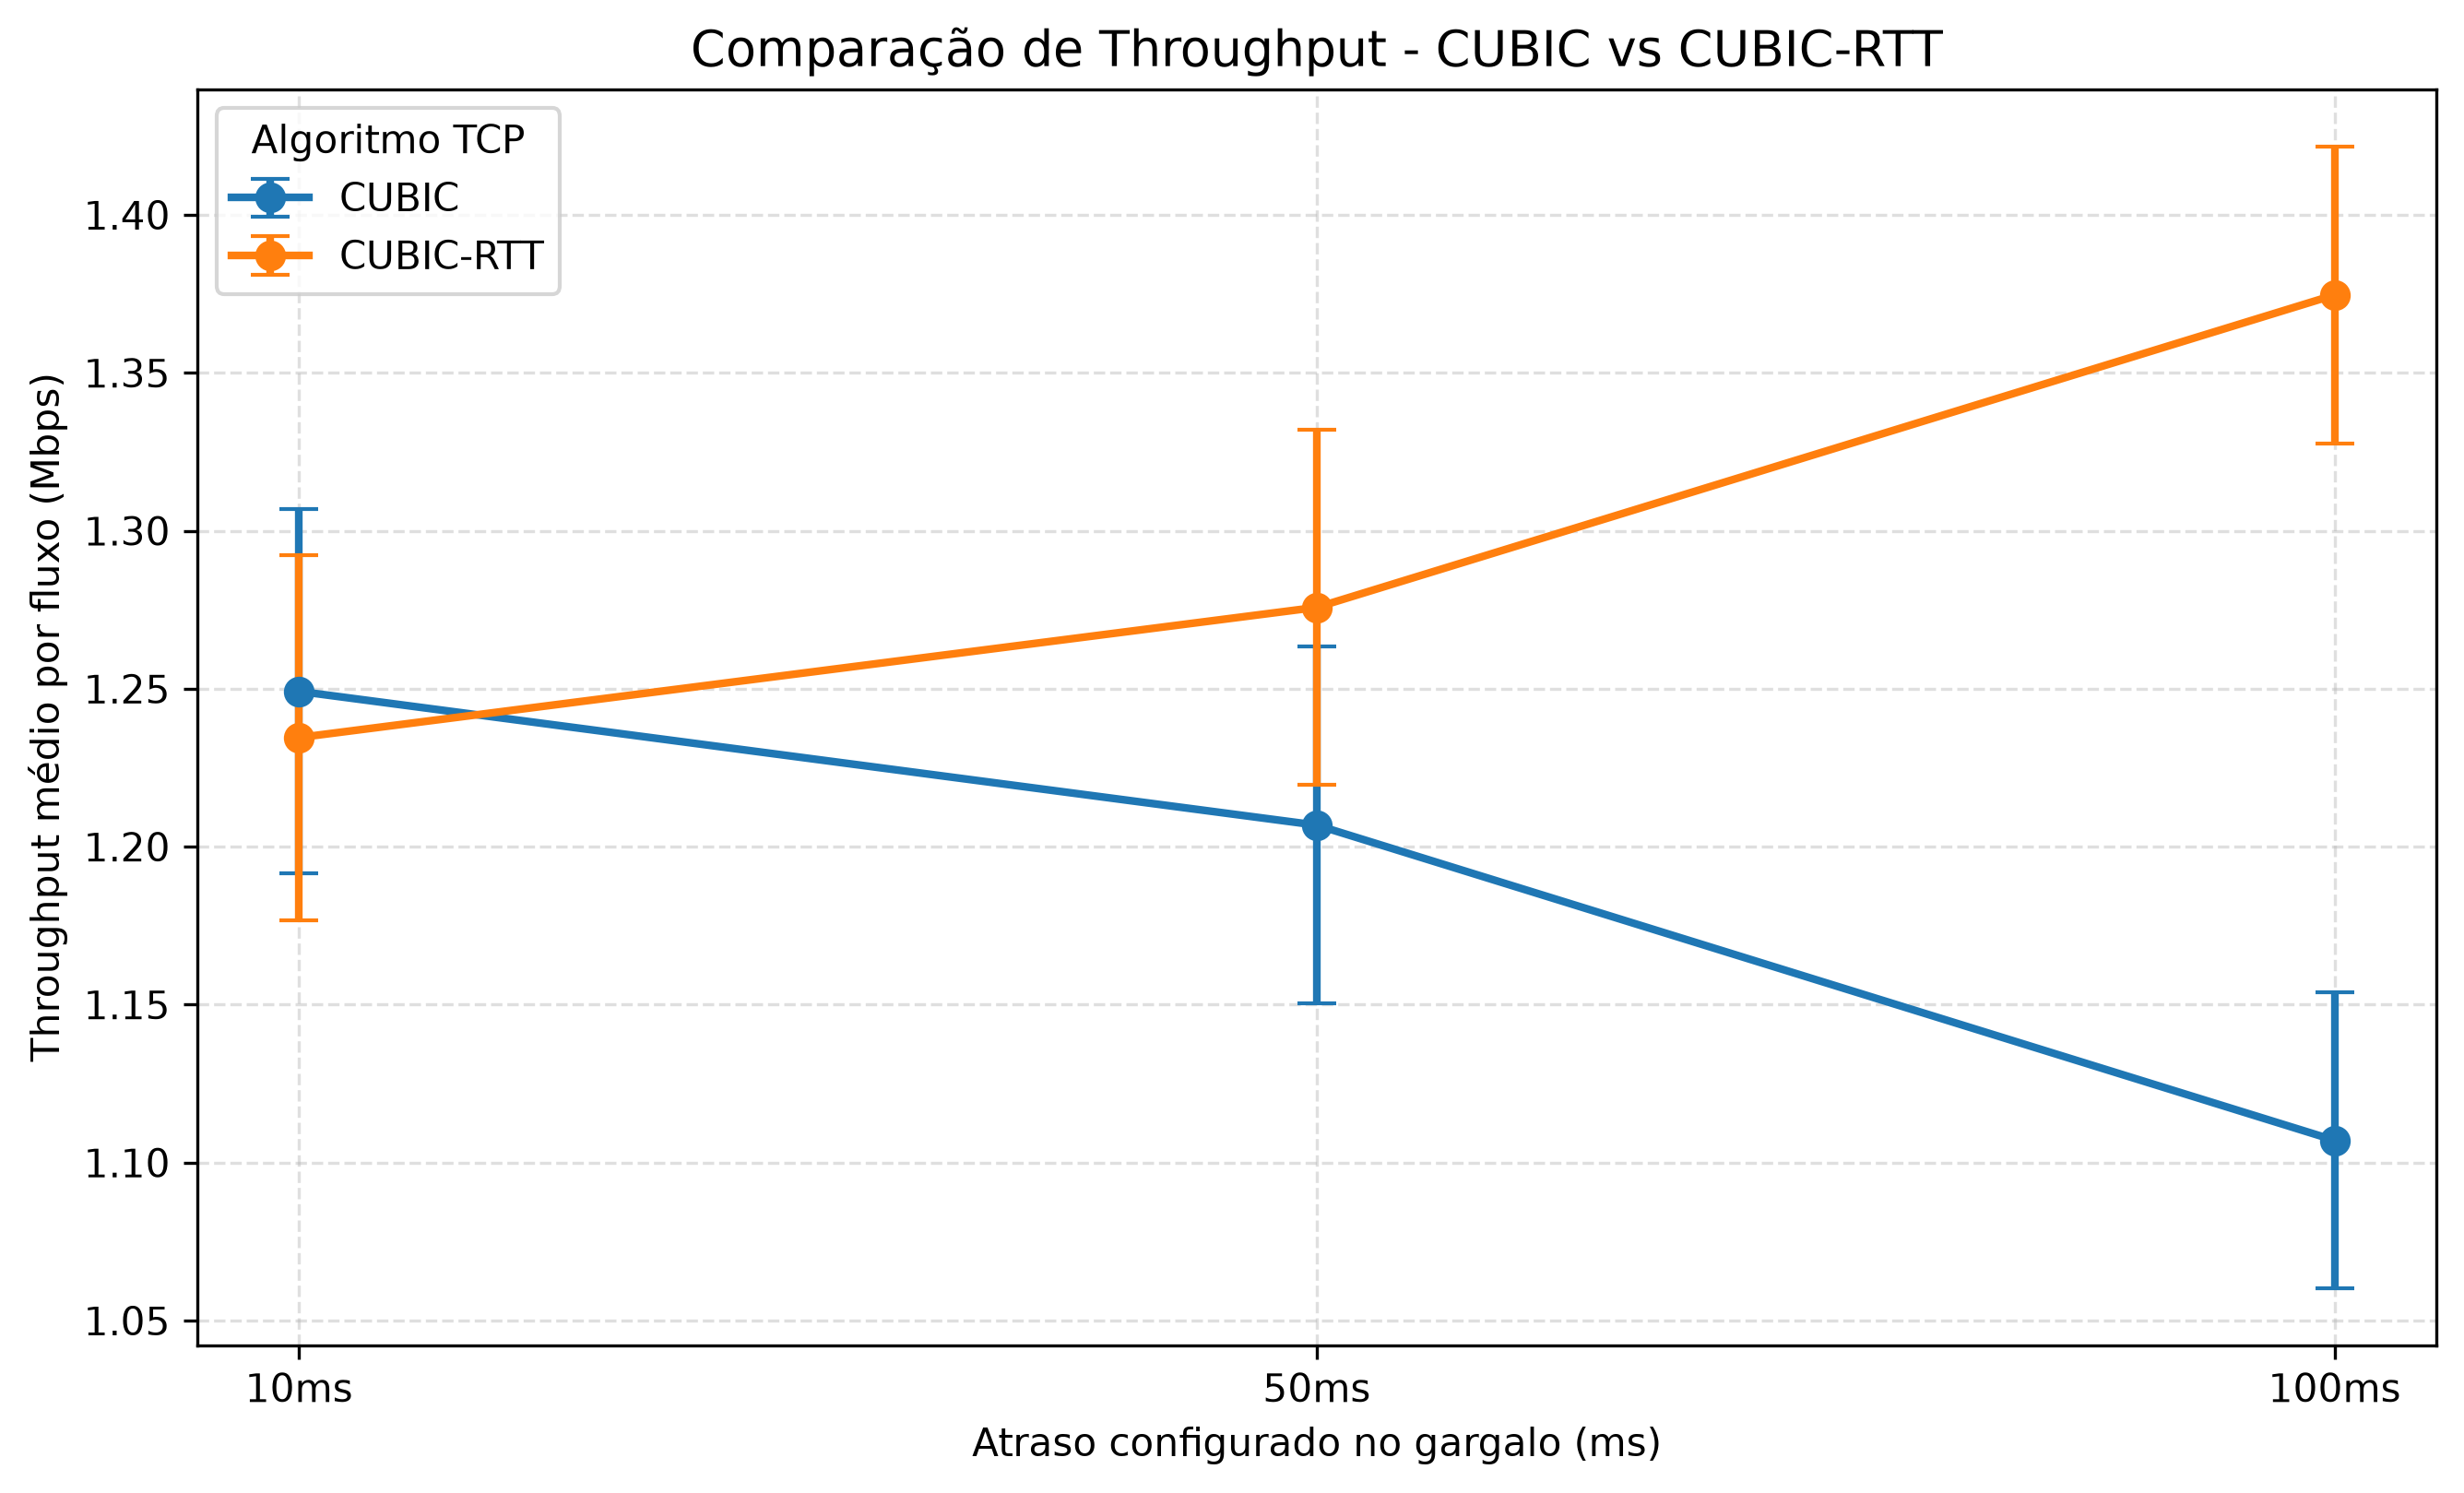
\includegraphics[width=0.90\textwidth]{01_throughput.png}
\caption{Vazão média por fluxo na campanha de coexistência.}
\label{fig:coex-throughput}
\end{figure}

\subsection{Atraso médio}

O atraso médio dos dois grupos permaneceu praticamente igual em todos os cenários. Em 10 ms, a diferença foi de aproximadamente 0,31 ms; em 50 ms, 0,17 ms; e em 100 ms, 0,49 ms. Essas diferenças são muito pequenas quando comparadas aos valores absolutos, que cresceram de aproximadamente 450 ms para 678 ms à medida que o atraso do gargalo aumentou.

Na prática, o ganho de vazão do CUBIC-RTT em 50 ms e 100 ms não foi acompanhado por uma redução expressiva do atraso médio. Os dois algoritmos experimentaram condições de atraso muito próximas, embora tenham obtido parcelas diferentes da vazão disponível.

\begin{figure}[htbp]
\centering
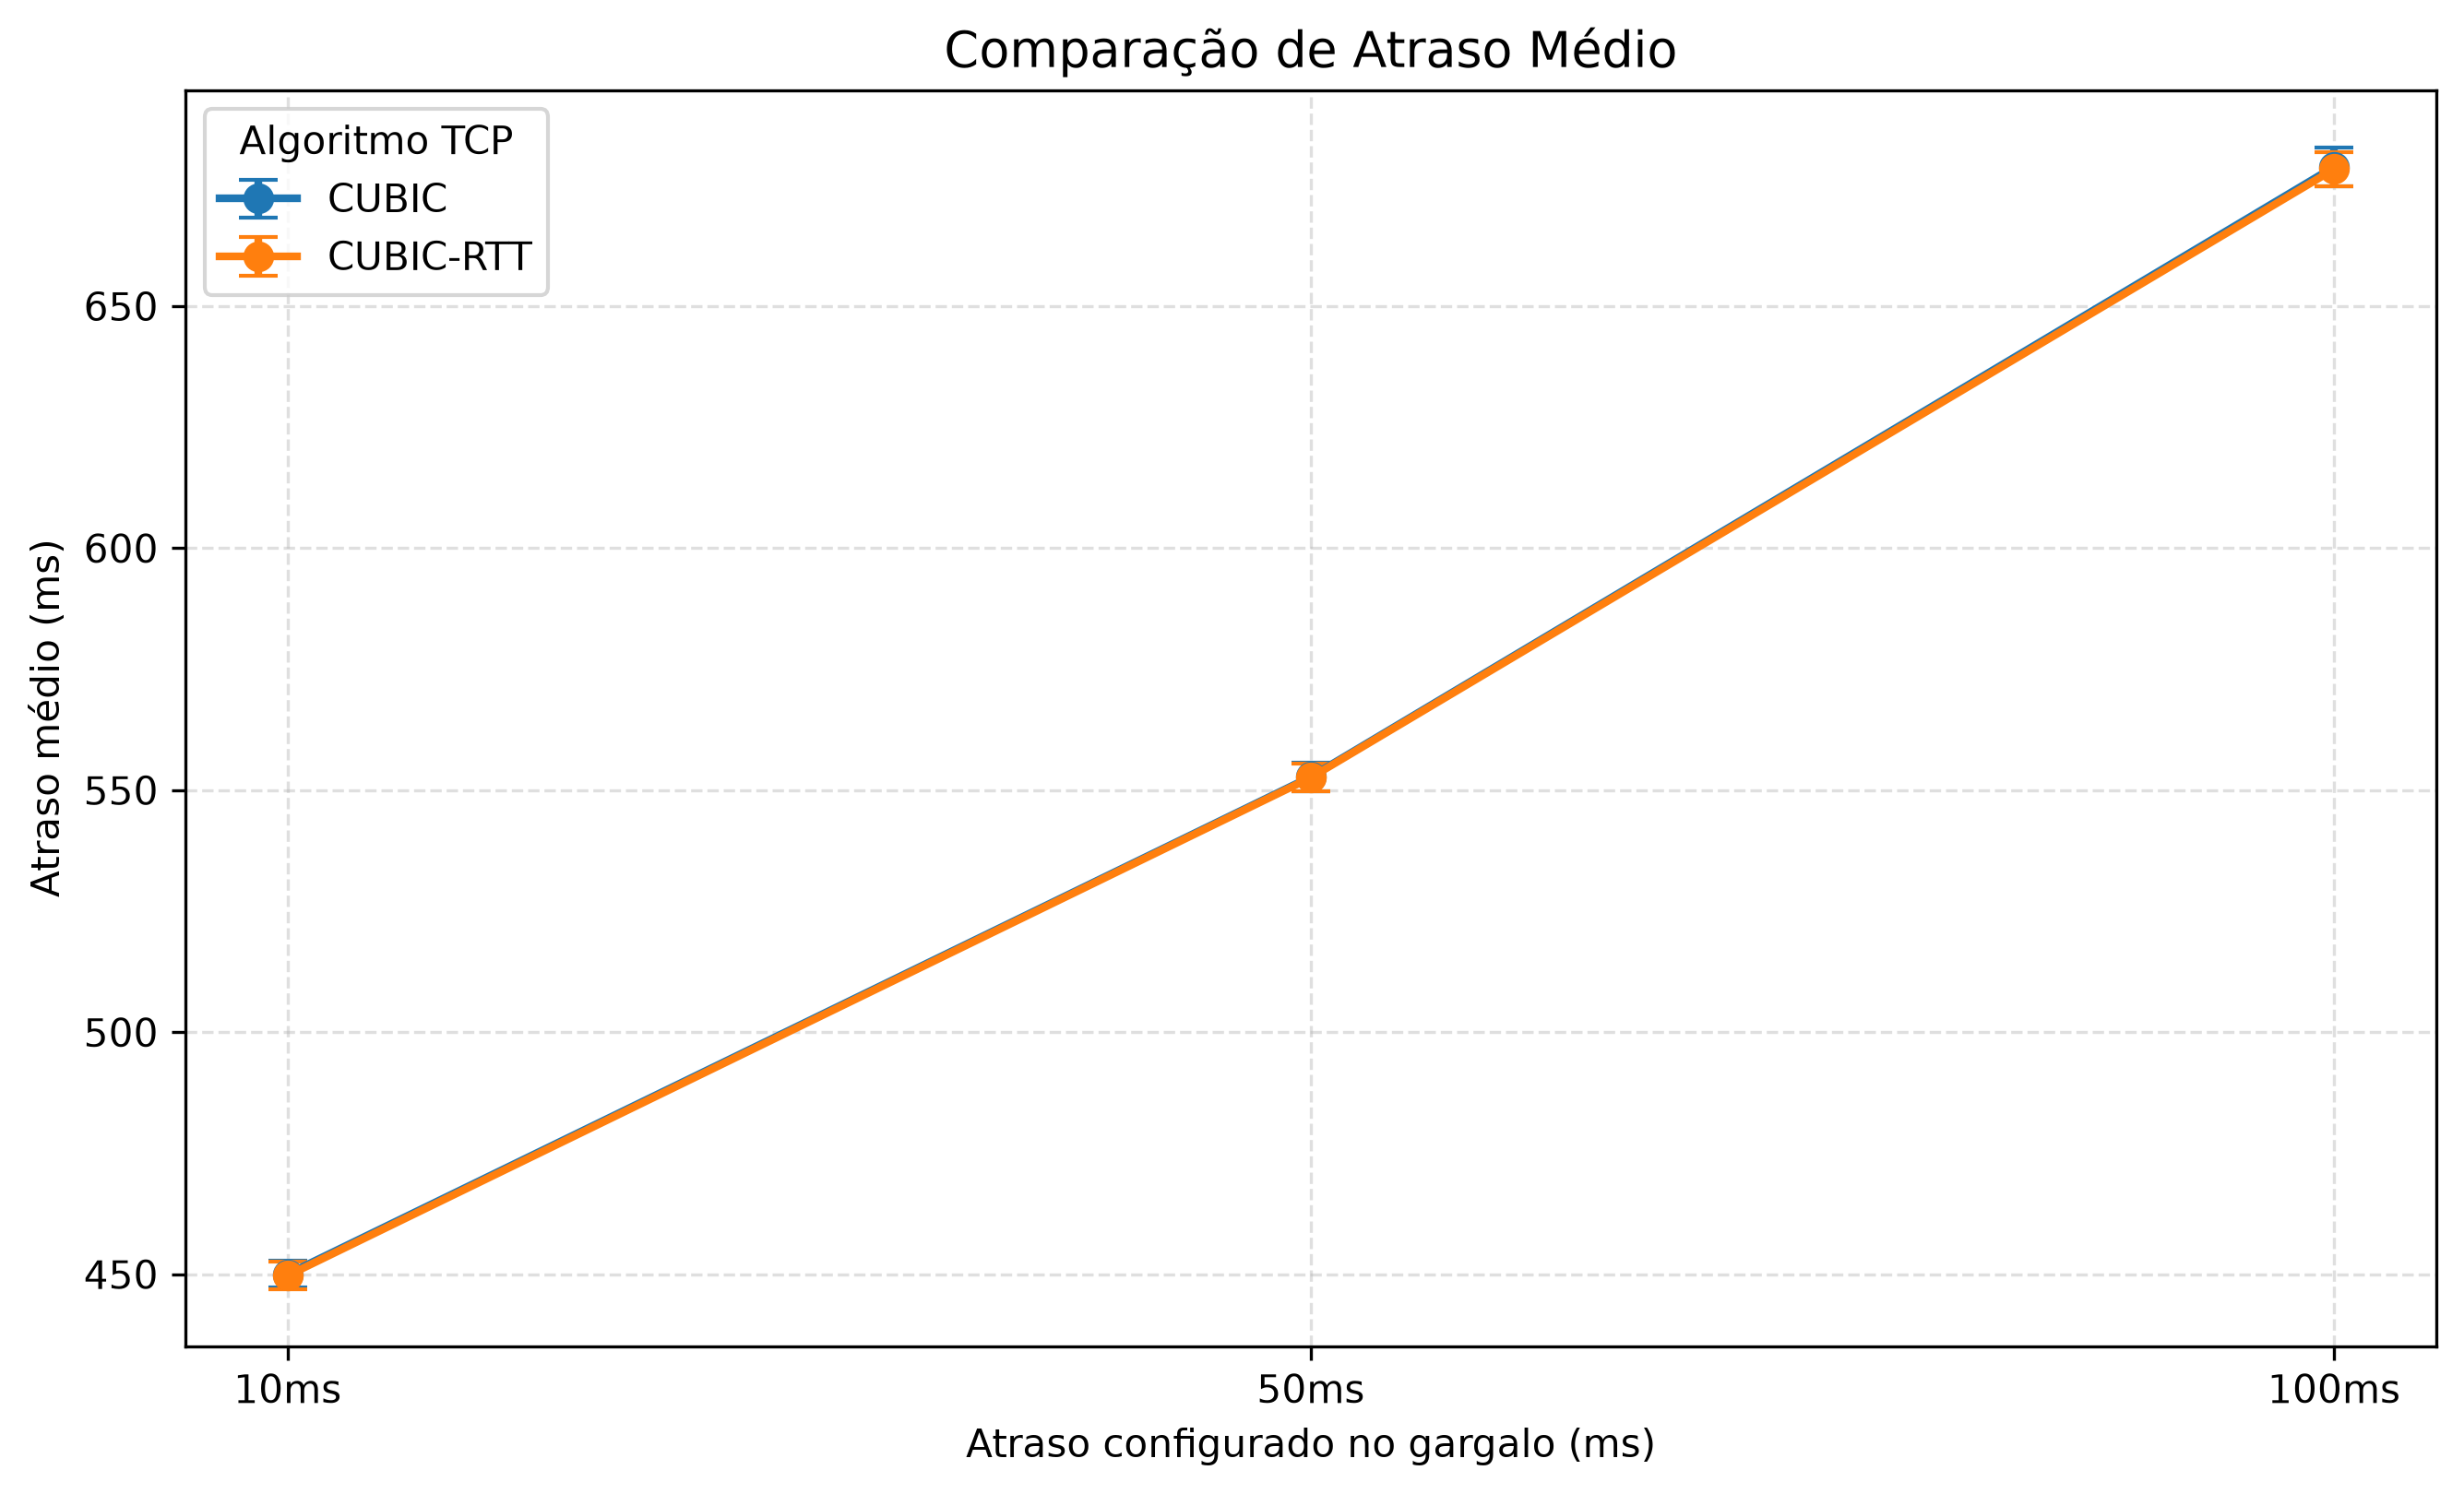
\includegraphics[width=0.90\textwidth]{02_atraso_medio.png}
\caption{Atraso médio dos fluxos na campanha de coexistência.}
\label{fig:coex-atraso}
\end{figure}

\subsection{Jitter e perda de pacotes}

No cenário de 10 ms, o jitter dos dois algoritmos foi praticamente igual: 0,6100 ms para CUBIC e 0,6131 ms para CUBIC-RTT. Em 50 ms, o jitter do CUBIC-RTT foi menor, 0,6380 ms contra 0,6487 ms. Em 100 ms, a diferença aumentou: 0,6556 ms para a proposta e 0,7060 ms para o CUBIC, uma redução aproximada de 7,1\%.

A perda de pacotes também foi ligeiramente menor para o CUBIC-RTT nos três atrasos. Em 10 ms, os valores foram 0,2416\% e 0,2465\%; em 50 ms, 0,3177\% e 0,3229\%; e em 100 ms, 0,4590\% e 0,5070\%. A diferença mais perceptível ocorreu no maior atraso, em que a perda do CUBIC-RTT ficou aproximadamente 9,5\% abaixo da observada no CUBIC.

\begin{figure}[htbp]
\centering
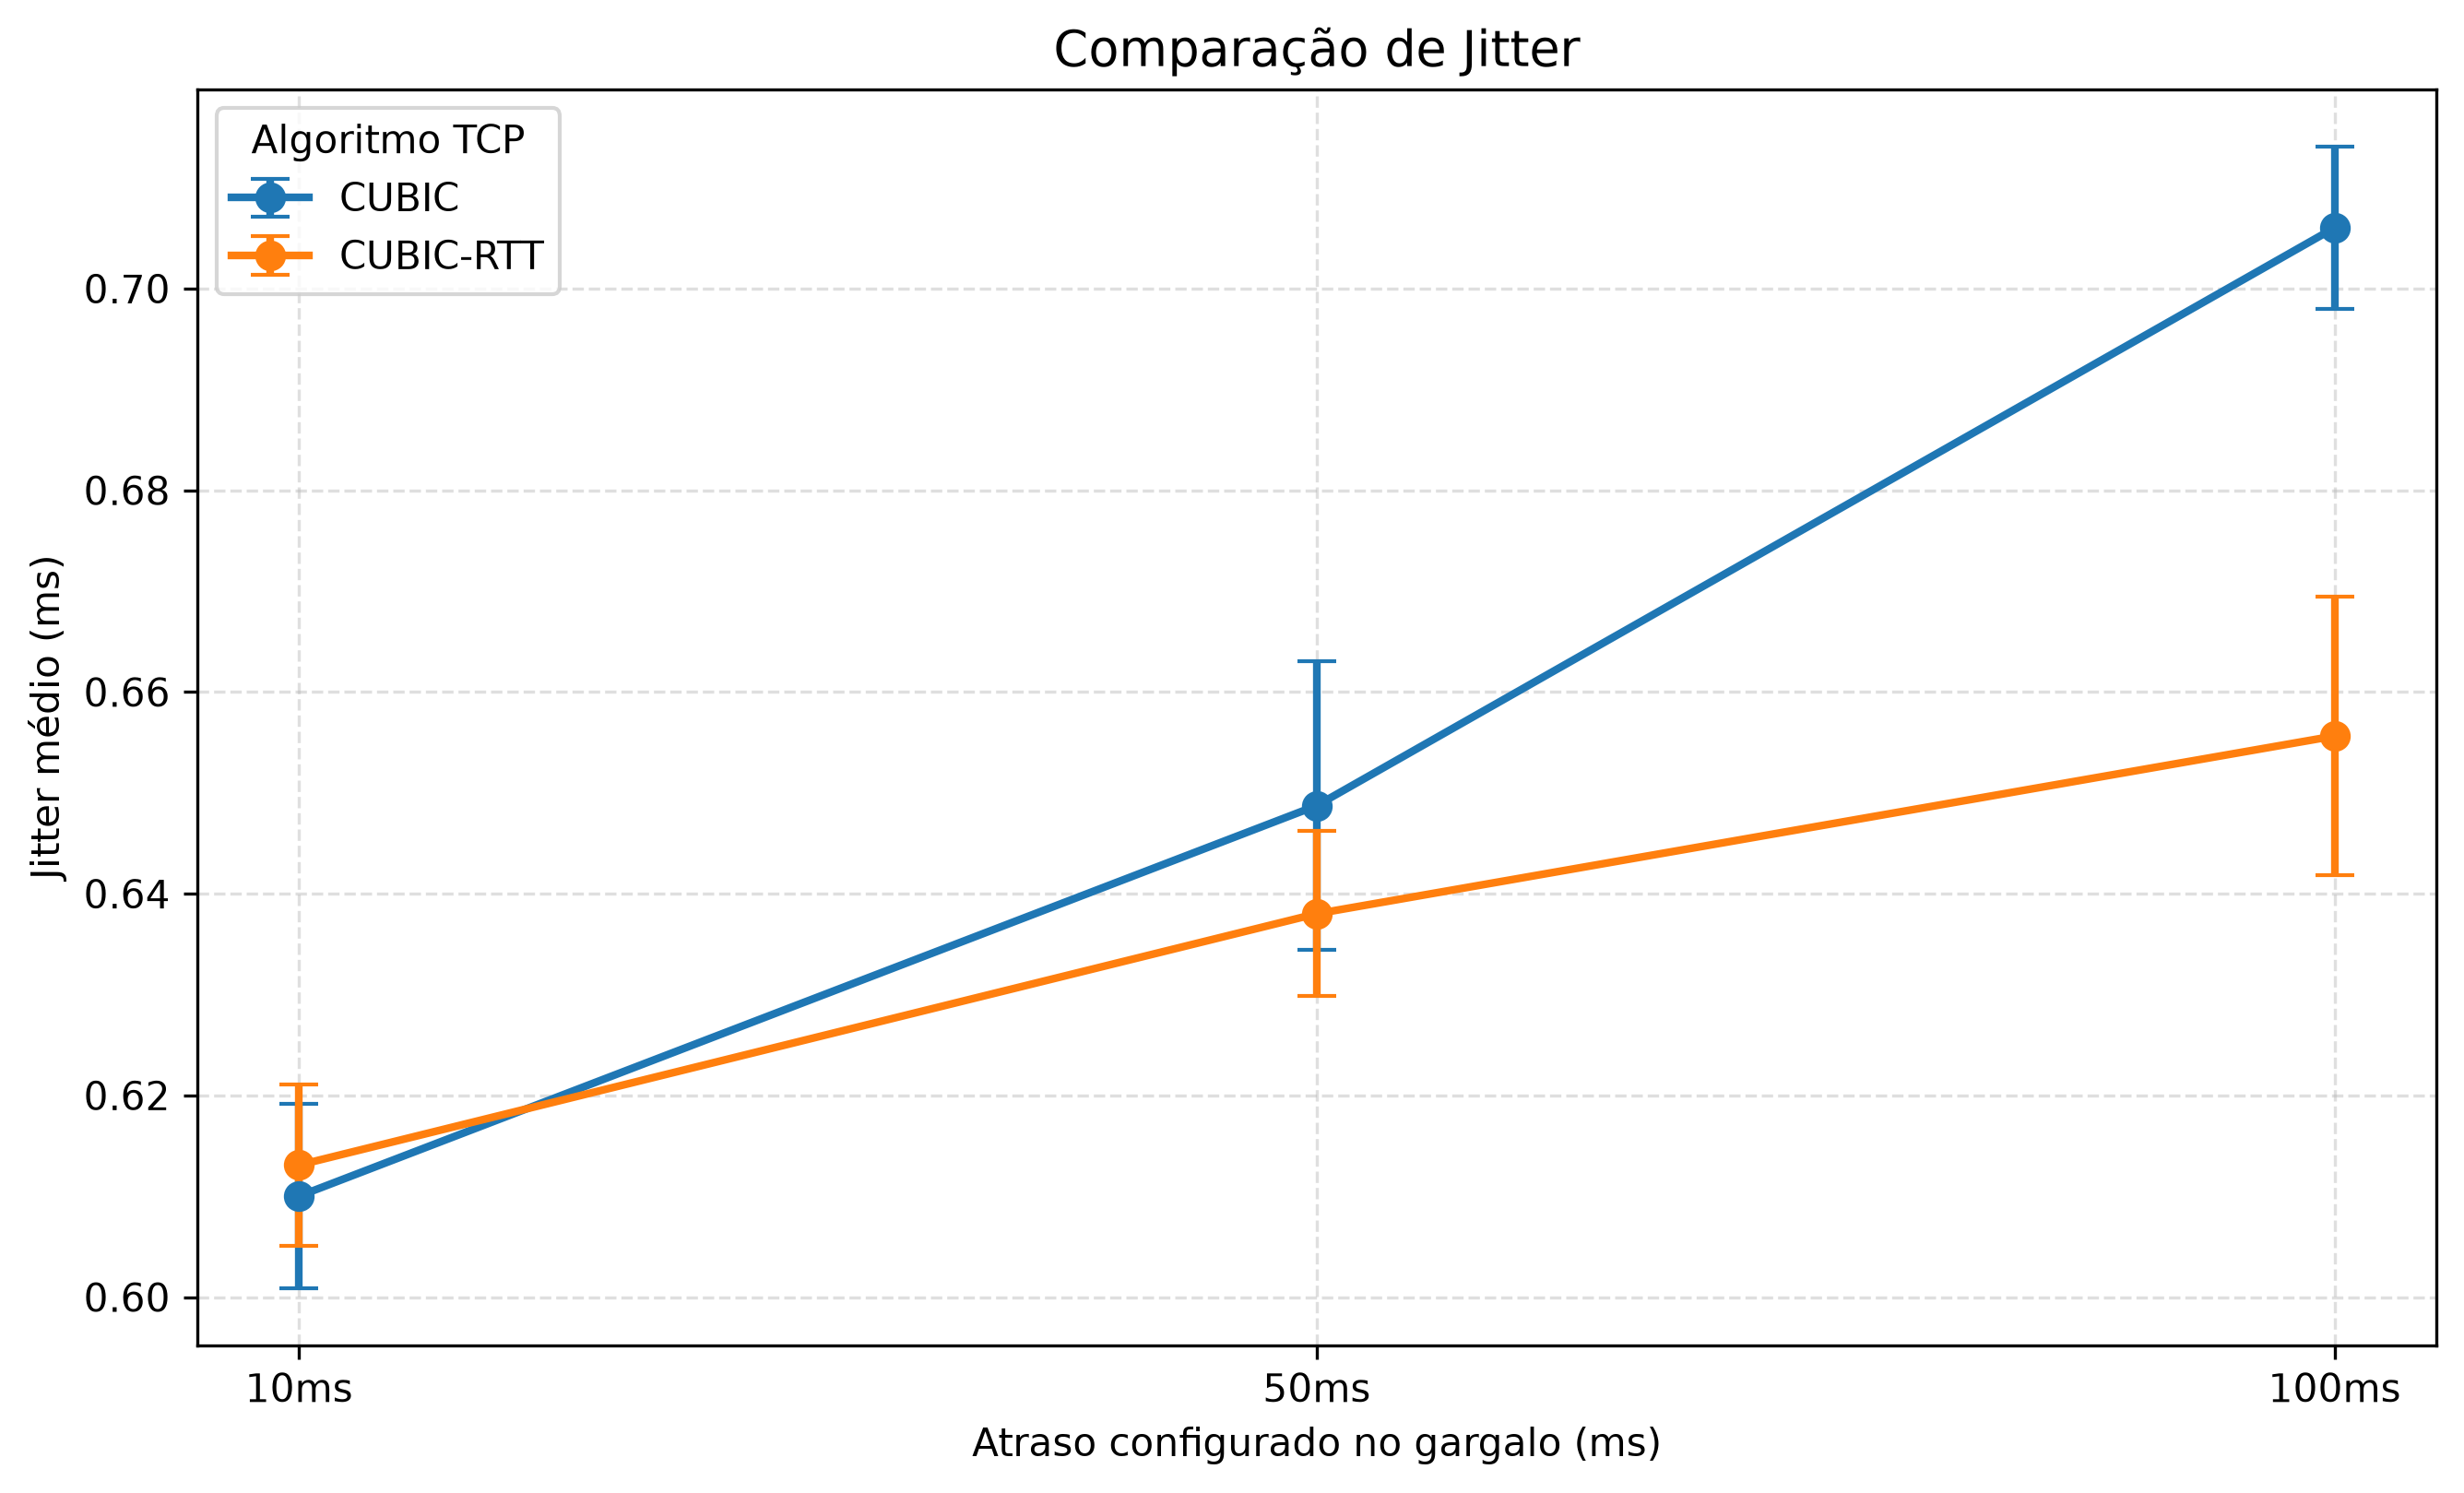
\includegraphics[width=0.90\textwidth]{03_jitter.png}
\caption{Jitter médio na campanha de coexistência.}
\label{fig:coex-jitter}
\end{figure}

\begin{figure}[htbp]
\centering
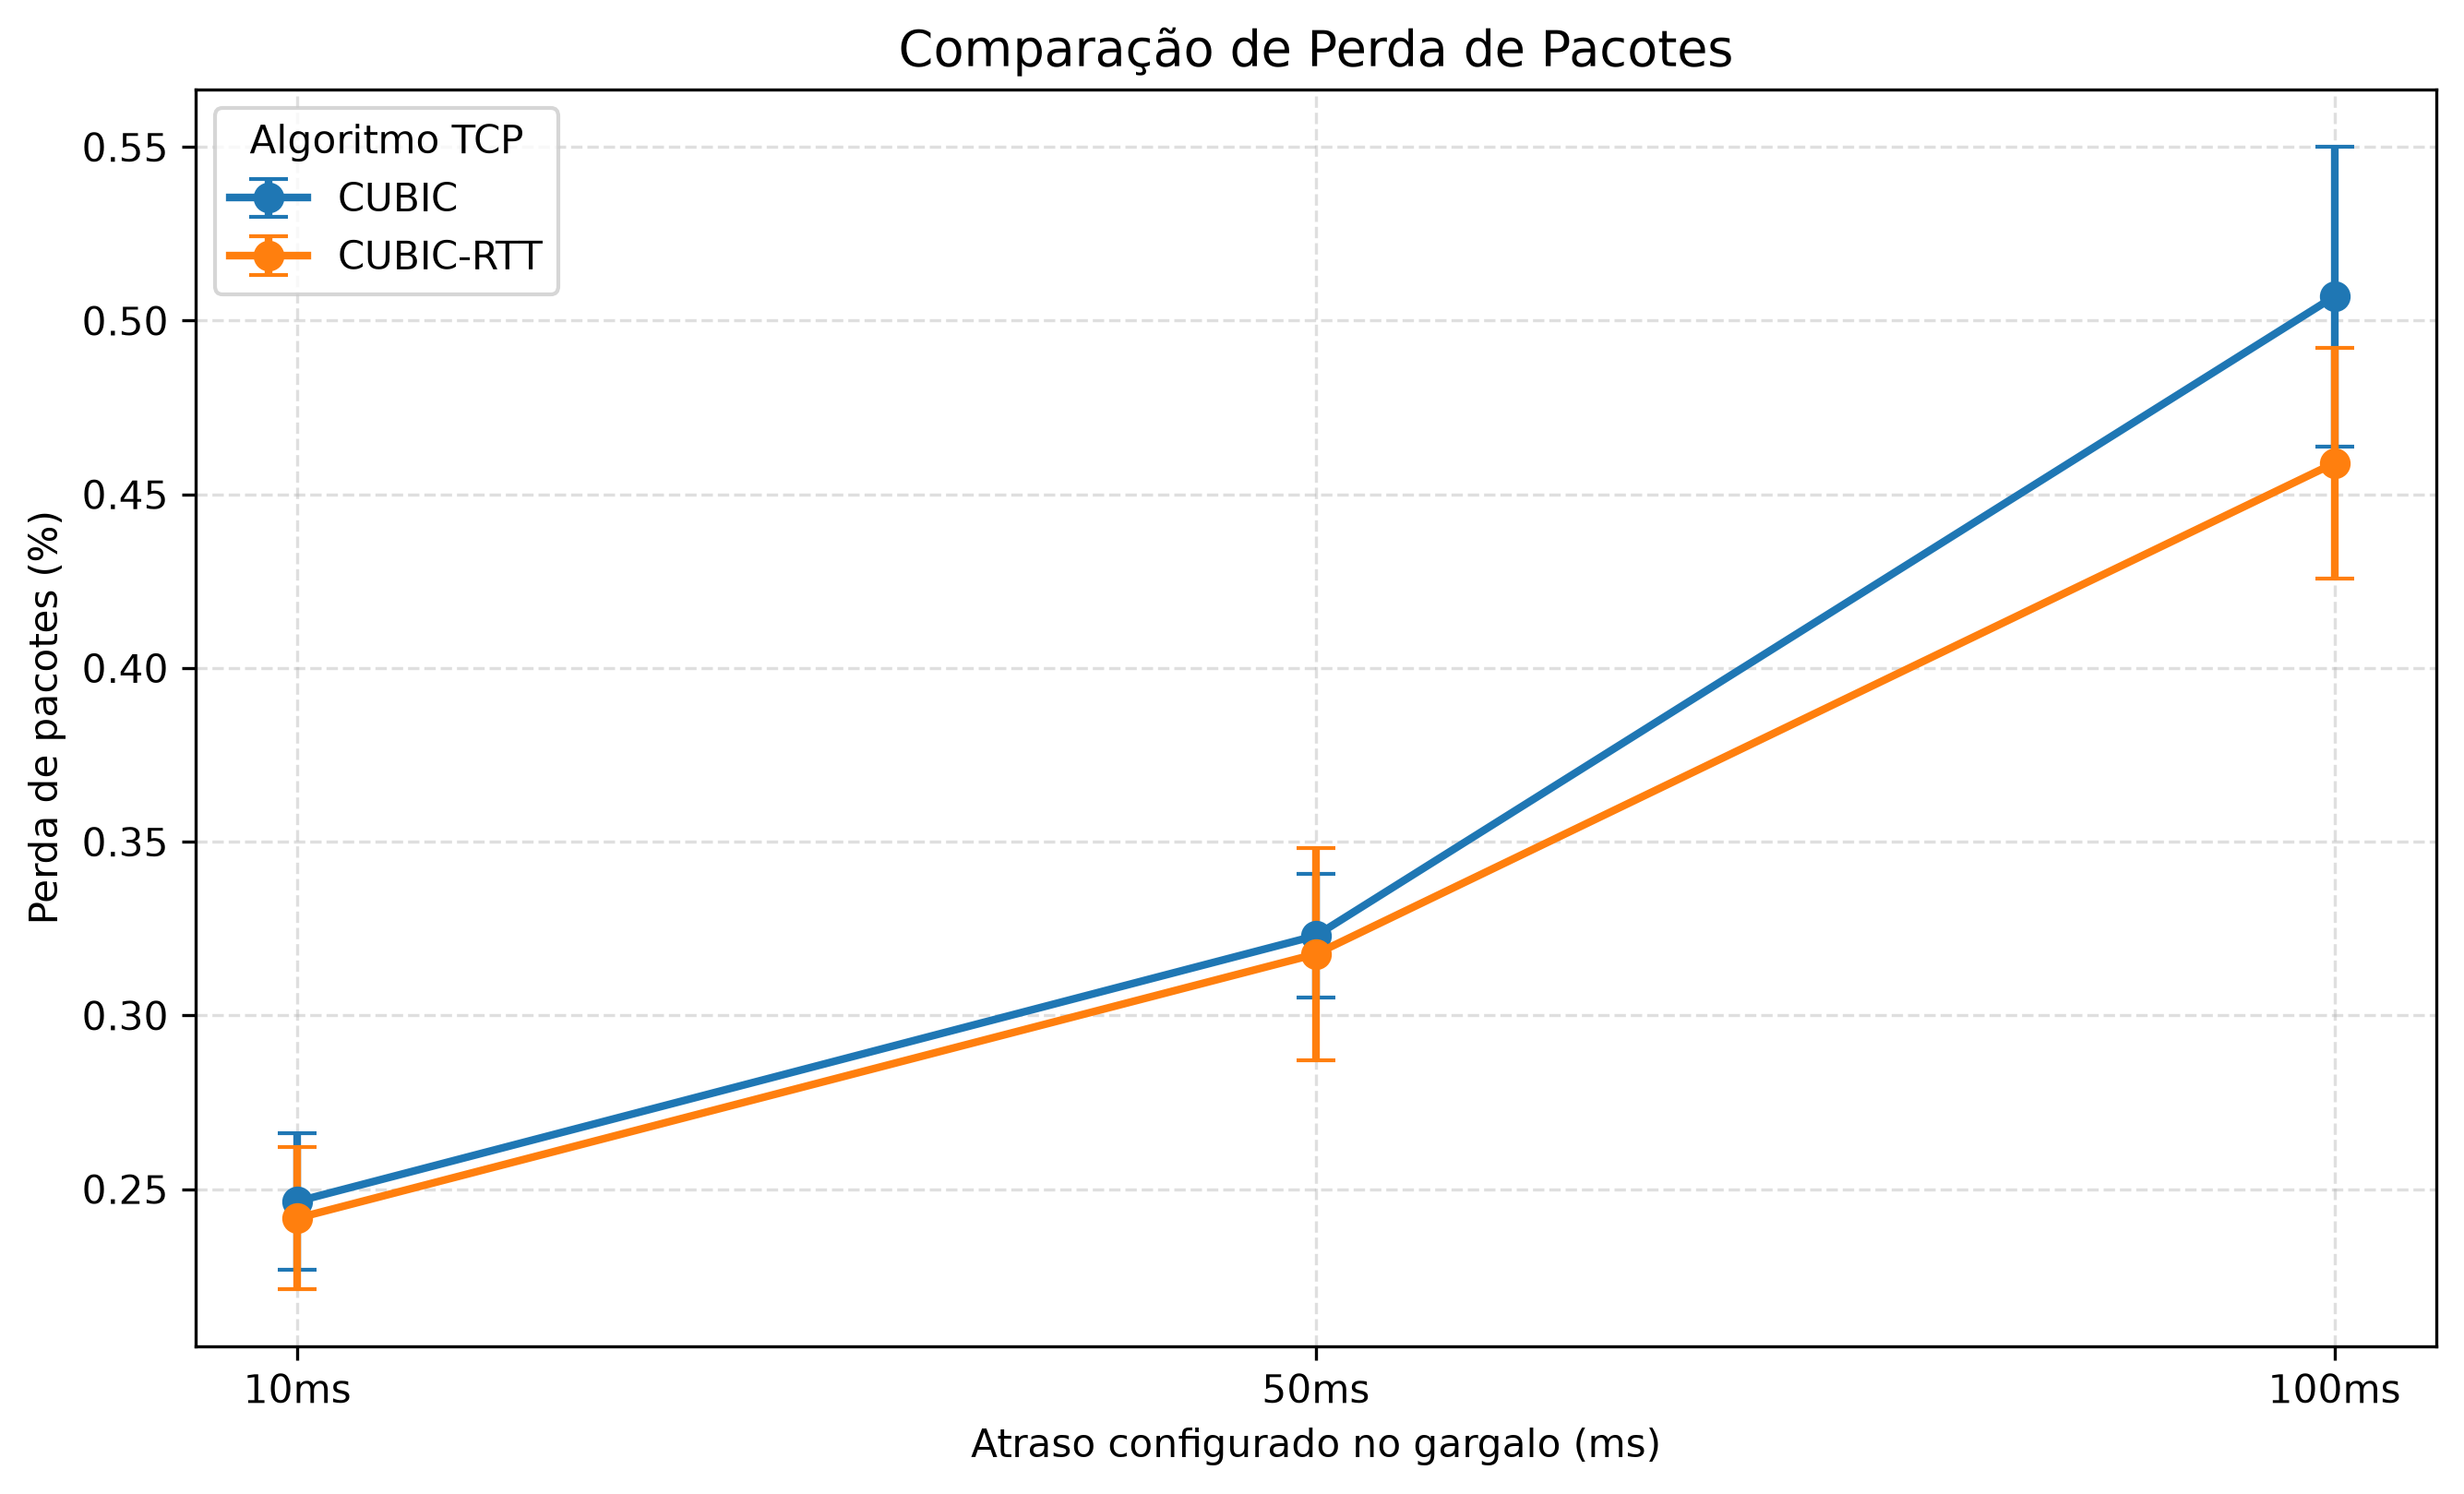
\includegraphics[width=0.90\textwidth]{04_packet_loss.png}
\caption{Taxa de perda de pacotes na campanha de coexistência.}
\label{fig:coex-perda}
\end{figure}

\subsection{Interpretação da coexistência}

A campanha mostra que o CUBIC-RTT consegue coexistir com o CUBIC sem derrubar a vazão total da rede e sem diferença expressiva no atraso médio. Coexistir, no entanto, não significa dividir os recursos igualmente: à medida que o atraso do gargalo aumentou, os fluxos CUBIC-RTT ficaram com uma fatia cada vez maior da capacidade, enquanto a vazão média dos fluxos CUBIC diminuiu.

Esse resultado sugere que a adaptação baseada em RTT dá à variante uma vantagem competitiva em cenários de maior atraso. A vantagem veio acompanhada de jitter e perda ligeiramente menores, mas não de uma redução significativa do atraso médio. Por isso, a proposta não deve ser descrita como uma simples melhoria de desempenho: ela muda a relação competitiva entre os algoritmos e pode favorecer quem a utiliza.

O ponto é relevante para a hipótese do trabalho. A informação de RTT mostrou-se útil para modificar a dinâmica do CUBIC, mas o experimento também deixa claro que uma adaptação vantajosa para os fluxos modificados pode reduzir a parcela de banda dos fluxos que continuam usando o algoritmo original. A avaliação da justiça entre algoritmos precisa, portanto, caminhar junto com a avaliação do desempenho individual.

\section{Análise das Variáveis Internas do TCP}

Os rastros de CWND, SSThresh, RTT, RTO e quantidade de dados em trânsito foram utilizados para observar a dinâmica das conexões ao longo das simulações. A auditoria estrutural confirmou 3.780 arquivos de CWND e 3.780 de SSThresh nas duas primeiras campanhas, sem pares ausentes, erros ou avisos.

Os gráficos temporais preservados para a campanha de coexistência mostram a evolução da janela de congestionamento e do RTT dos oito fluxos nos três atrasos de gargalo. As curvas apresentam fases iniciais de crescimento, seguidas de oscilações associadas à operação do controle de congestionamento. Com o aumento do atraso, a escala temporal do RTT se desloca para valores maiores, enquanto a janela continua apresentando variações ao longo da execução.

Esses rastros ajudam a interpretar as métricas agregadas, mas não devem ser usados isoladamente para afirmar que um algoritmo é melhor. Sua principal utilidade é permitir relacionar a evolução da janela e do RTT com as diferenças de vazão, jitter e perda observadas no FlowMonitor. Os gráficos representativos são reunidos no Apêndice~\ref{ap:traces}.

\section{Discussão Geral}

As três campanhas mostram aspectos complementares da proposta. Na comparação inicial, o CUBIC-RTT manteve a vazão agregada próxima à do CUBIC e reduziu moderadamente o jitter, mas apresentou atraso médio maior e perda ligeiramente superior nos cenários de maior atraso. Na campanha de robustez, a vazão permaneceu próxima da capacidade do gargalo, enquanto as demais métricas variaram de acordo com o cenário e com os valores de $\alpha$ e $\gamma$. Não houve uma configuração que apresentasse o melhor resultado em todas as métricas.

A campanha de coexistência acrescentou um resultado importante: quando CUBIC e CUBIC-RTT compartilham o mesmo gargalo, a variante adaptativa pode obter uma parcela maior da vazão, especialmente quando o atraso do gargalo aumenta. Esse ganho não elevou a vazão total da rede, que permaneceu próxima de 10 Mbps; ele alterou a distribuição da capacidade entre os grupos de fluxos.

Em relação à hipótese de partida, os experimentos sustentam que informações de RTT podem ser incorporadas à estrutura do CUBIC e modificar seu comportamento. Já a expectativa de que essa alteração produza, em qualquer cenário, menor atraso, maior justiça e manutenção integral do desempenho dos fluxos concorrentes não foi confirmada. O resultado mais adequado é considerar o CUBIC-RTT uma variante experimental com efeitos dependentes do cenário e com um compromisso claro entre regularidade, perda e competitividade.
